\section{Verfahrensvergleich}
\label{sec:verfahrensvergleich}
Wir werden nun die numerischen Verfahren zur Lösung von Anfangswertproblemen mit dem Verfahren der Lösungspakete
vergleichen. Es werden hierfür die Python Bibliotheken \textit{numpy} 1.21.4, \textit{scipy} 1.7.2 für numerische
Verfahren und \textit{tensorflow} 2.7.0 für die Architektur der neuronalen Netze verwendet. Das gegebene
Anfangswertproblem wird zuerst mithilfe des \textit{4-5-Runge-Kutta-Verfahren} beziehungsweise einem BDF-Verfahren
gelöst und danach mit einem neuronalen Netz approximiert. Die folgenden Ergebnisse werden darauffolgend mit
verschiedenen Fehlermaßen verglichen. Die Berechnungen wurden mit einem AMD Ryzen 7 5800X CPU, 32GB RAM und einer
NVIDIA RTX 3060 Ti GPU durchgeführt.

\subsection{Rebound-Pendel}
\label{subsec:rebound-Pendel}
Ein Rebound-Pendel ist ein System, in dem ein Pendel an einer Seite auf eine gedämpfte Feder treffen kann.
\begin{figure}
       \centering
       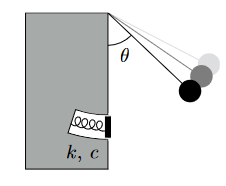
\includegraphics{rebound_pendulum_diagram}
       \caption{Diagramm eines Rebound Pendels\cite[6]{flamantSolvingDifferentialEquations2020}}
       \label{fig:rebound_pendulum_diagram}
\end{figure}
Ein Beispiel des beschriebenen Systems wird in Abbildung \ref{fig:rebound_pendulum_diagram} gezeigt. Das zugehörige
Anfangsproblem 2. Ordnung hat die Form
\begin{align*}
       \theta^{\prime \prime} &= - \frac{g}{l} \sin(\theta) + H(-\theta)
       \text{ReLU}(-\frac{kl}{m}\theta - c \theta^{\prime})\\
       \theta(0) &= 1, \quad \theta^{\prime}(0)=0.2,
\end{align*}
beziehungsweise mit der Einführung einer weiteren Variable $\varphi=\theta^{\prime}$ zu einem System erster Ordnung
\begin{align}
       \theta^{\prime} &= \varphi \nonumber \\
       \varphi^{\prime} &= - \frac{g}{l} \sin(\theta) + H(-\theta)
       \text{ReLU}(-\frac{kl}{m}\theta - c \varphi) \label{rebound-pendulum}\\
       \theta(0) &= 1, \quad \varphi(0)=0.2. \nonumber
\end{align}
Hierbei ist $\text{ReLU}(x)= \max(x, 0)$,
\begin{align*}
       H(x) =
       \begin{cases}
              0, &x<0 \\
              1, &x \geq 0
       \end{cases},
\end{align*}
$g$ die Erdbeschleunigung, $l$ die Länge des Pendels, $m$ die Masse des Pendels, $k$ die Federkonstante und $c$ der
Dämpfungskoeffizient. Wir werden dieses System nun in dem Zeitraum $t \in [0, 10]$ lösen bzw. approximieren und die
Resultate vergleichen. Für beide Verfahren werden zur Vereinfachung $g=1$ und $l=1$ gesetzt. Außerdem gilt für das
Runge-Kutta-Verfahren $k=3$ und $c=1$.
\begin{table}
              \renewcommand{\arraystretch}{1.0}
              \centering
              \begin{tabular}{ l | l }
                     \hline
                     Netzwerkstruktur & \\
                     \hline
                     Anzahl der Schichten & $L=10$ \\
                     Eingabeschicht & $n^{(0)}=5$ mit $\Phi(x)=\tanh(x)$ \\
                     versteckte Schichten & $n^{(l)}=128$, $l = 1, \dots, L-1$ mit $\Phi(x)=\tanh(x)$ \\
                     Ausgabeschicht & $n^{(L)}=2$ mit $\Phi(x)=x$ \\
                     \hline
                     Hyperparameter und Initialisierungsintervalle & \\
                     \hline
                     Anfangswertbereiche & $(\theta_0, \varphi_0) \in [0.0, 1.0] \times [-0.2, 0.2]$ \\
                     Paramaterbereiche & $(k, c) \in [2.0, 5.0] \times [0.0, 2.0]$ \\
                     Zeitraum & $t \in [0, 10]$ \\
                     \hline
                     Optimierung & \\
                     \hline
                     Gradientenverfahren & Adam \\
                     Gewichtsfunktion & $b(t)=e^{-0.5t}$ \\
                     Batchsize & $|B|=10000$ \\
                     Epochen & $1000000$ \\
                     Learning rate & $\eta= 0.0001$ \\
                     Gewichtsinitialisierung & Xavier-Initialisierung \\
                     \hline
                     Statistiken & \\
                     \hline
                     Trainingrate & xx \\
                     Traningszeit & xx Stunden \\
                     \hline
              \end{tabular}
       \caption{Netzwerkstruktur, Hyperparameter, Initialisierungsintervalle, Optimierungsparameter und Statistiken
       für das Rebound-Pendel-Anfangswerproblem.}
       \label{rebound-pendulum-table}
\end{table}
In Tabelle \ref{rebound-pendulum-table} sind alle relevanten Daten für das Rebound-Pendel-Anfangswerproblem gegeben,
wobei $\Phi(x)$ die Aktivierungsfunktion für die jeweiligen Schichten ist. Da die rechte Seite $f$ von
\eqref{rebound-pendulum} nicht differenzierbar ist, lässt sich keine einfache Schlussfolgerung für die Existenz und
Eindeutigkeit der exakten Lösung formulieren. Da wir keine exakte Lösung $x$haben,ist es nicht möglich, die beiden
Verfahren durch den globalen Fehler $\left\lVert u - x \right\rVert_2$ zu vergleichen, wobei $u$ das Ergebnis des
zugehörigen Verfahrens ist. Außerdem ist ein Vergleich der Trajektorien zu ungenau um qualitative Aussagen über die
Effizienz liefen zu können. Wir konstruieren nun also ein Fehlermaß, um die Verfahren vergleichen zu können.
!!TODO: Graphiken und atol,rtol!!

\subsection{Steife Differentialgleichung}
\label{sec:steife-differentialgleichung}
Die Anfangswertproblem
\begin{align}
       \label{stiff}
       x_{1}^{\prime} &= \frac{1}{2} ((\lambda_1 + \lambda_2)x_1 + (\lambda_1 - \lambda_2)x_2), \nonumber \\
       x_{2}^{\prime} &= \frac{1}{2} ((\lambda_1 - \lambda_2)x_1 + (\lambda_1 + \lambda_2)x_2), \\
       x_1(0) &= c_1 + c_2, \quad x_2(0) = c_1 - c_2 \nonumber
\end{align}
lässt sich mit der Matrix
\[
       A = \frac{1}{2}
       \begin{bmatrix}
                \lambda_1 + \lambda_2 & \lambda_1 - \lambda_2 \\
                \lambda_1 - \lambda_2 & \lambda_1 + \lambda_2
       \end{bmatrix}
\]
zu
\begin{align*}
       x^{\prime} &= Ax, \\
       x(0) &=
       \begin{bmatrix}
              c_1 + c_2 \\
              c_1 - c_2
       \end{bmatrix}
\end{align*}
umformulieren. Dabei gilt $\lambda_1, \lambda_2 < 0$ und $c_1, c_2 \in \mathbb{R}$. A hat die Eigenwerte
$\lambda_1(A) = \lambda_1$ und $\lambda_2(A) = \lambda_2$ und für $\lambda_1 = -100$ und $\lambda_2 = -1$ ist
das Anfangswertproblem \eqref{stiff} nach Definition \eqref{steife-dgl} $steif$. Da \eqref{stiff} eine lineare
Differentialgleichung erster Ordnung ist, können wir die Lösung mithilfe \eqref{linear-ode-solution} angeben:
\[
       x(t) =
       \begin{bmatrix}
              c_1 e^{\lambda_1 t} + c_2 e^{\lambda_2 t} \\
              c_1 e^{\lambda_1 t} - c_2 e^{\lambda_2 t}
       \end{bmatrix}.
\]
Der erste Eigenwert $\lambda_1$ lässt den ersten Summand der Lösung viel schneller gegen $0$ konvergieren für
$t \rightarrow \infty$, als der zweite Eigenwert $\lambda_2$. Verwenden wir nun das explizite Euler-Verfahren mit der
Form
\begin{align*}
       u_0 &= x_0 \\
       u_i &= u_{i-1} + hAu_{i-1}= \dots = (I + hA)^{i}u_0, \qquad i=1,\dots,N
\end{align*}
um das Anfangswertproblem zu lösen. Die numerische Lösung ist also gegeben mit
\begin{align*}
       u_{i}=
       \begin{bmatrix}
              c_1 (1+h\lambda_1)^{i} + c_2 (1+h\lambda_2)^{i}\\
              c_1 (1+h\lambda_1)^{i} + c_2 (1+h\lambda_2)^{i}
       \end{bmatrix}.
\end{align*}
Damit die exakte Lösung und die numerische Lösung das gleiche Grenzverhalten besitzen, muss $|1 + h\lambda_1|<1$ und
$|1 + h\lambda_2|<1$ gelten. Hieraus resultieren Bedinungen für $h$, also eine Schrittweitenbeschränkung der Form
$h<\frac{2}{|\lambda_1}$ und $h<\frac{2}{\lambda_2}$. Da $|\lambda_2| \ll |\lambda_1|$, bestimmt der erste Eigenwert
über die Beschränkung der Schrittweite, obwohl dieser in der exakten Lösung für größere Zeiten $t$ fast keinen Einfluss
hat. Wir werden sehen, dass dieses Problem auch für Runge-Kutta-Verfahren auftreten, weshalb wir außerdem ein
\textit{BDF-Verfahren}, also ein Mehrschrittverfahren, verwenden werden, um die Ergebnisse mit dem Verfahren der
Lösungspakete vergleich zu können. Für alle Verfahren setzen wir $c_1=3$, $c_2=4$, $\lambda_1 = -100$ und $\lambda_2=-1$.
Es wird die Bibliothek $scipy.integrate$, genauer die Funktionen $scipy.integrate.RK45$ (Dokumentation siehe
\cite{ScipyIntegrateRK45}) für ein Runge-Kutta-Verfahren und $scipy.integrate.BDF$ (Dokumentation siehe
\cite{ScipyIntegrateBDF}) verwendet. Für beide Verfahren setzen wir dazu die relative Toleranz $rtol=10^{-2}$
und die absolute Toleranz $atol=10^{-7}$ um die Steiffheit des gegebenen Anfangswertproblems \eqref{stiff} beobachten
zu können. Ähnlich wie in Abschnitt \ref{subsec:rebound-Pendel} sind in Tabelle \ref{stiff-table} alle relevanten Daten
zu dem verwendeten neuronalen Netz \eqref{stiff} gegeben.
\begin{table}
       \renewcommand{\arraystretch}{1.0}
       \centering
       \begin{tabular}{ l | l }
              \hline
              Netzwerkstruktur & \\
              \hline
              Anzahl der Schichten & $L=10$ \\
              Eingabeschicht & $n^{(0)}=5$ mit $\Phi(x)=\tanh(x)$ \\
              versteckte Schichten & $n^{(l)}=32$, $l = 1, \dots, L-1$ mit $\Phi(x)=\tanh(x)$ \\
              Ausgabeschicht & $n^{(L)}=2$ mit $\Phi(x)=x$ \\
              \hline
              Hyperparameter und Initialisierungsintervalle & \\
              \hline
              Anfangswertbereiche &
              $x_{1,0} \in [c_1+c_2 - 0.05, c_1+c_2 + 0.05]$ \\
              & $x_{2,0} \in [c_1-c_2 - 0.05, c_1-c_2 + 0.05]$ \\
              Paramaterbereiche &
              $\lambda_1 \in [\lambda_1 - 0.05, \lambda_1 + 0.05]$ \\
              & $\lambda_2 \in[\lambda_2 - 0.05, \lambda_2 + 0.05]$ \\
              Zeitraum & $t \in [0, 10]$ \\
              \hline
              Optimierung & \\
              \hline
              Gradientenverfahren & Adam \\
              Gewichtsfunktion & $b(t)=e^{-0.5t}$ \\
              Batchsize & $|B|=10000$ \\
              Epochen & $1000000$ \\
              Learning rate & $\eta= 0.0001$ \\
              Gewichtsinitialisierung & Xavier-Initialisierung \\
              \hline
              Statistiken & \\
              \hline
              Trainingrate & 125 Batches/Sekunde \\
              Traningszeit & 2,22 Stunden \\
              \hline
       \end{tabular}
       \caption{Netzwerkstruktur, Hyperparameter, Initialisierungsintervalle, Optimierungsparameter und Statistiken
       für das steife Anfangswertproblem \eqref{stiff}.}
       \label{stiff-table}
\end{table}
!!TODO: Grafiken!!
In Abbildung \ref{fig:stiff-trajectories} können wir den Verlauf der Trajektorie mit dem Anfangspunkt
$x_0=x(0)=(7,-1)^{\intercal}$ für die erwähnten Verfahren betrachten. Wie bereits besprochen beschränkt der betragsmäßig große
Eigenwert $\lambda_1=-100$ die Schrittweite $h$, was zu einer ungenauen Lösung des Runge-Kutta-Verfahren führt. Die
Approximation des neuronalen Netzes jedoch lässt sich mit der Perfomance des BDF-Verfahrens vergleichen, da es für ein
Zeitintervall sogar bessere Ergebnisse liefert als das BDF-Verfahren.
Dieses Verhalten lässt sich auch in der Abbildung des Fehlers in Abhängigkeit der Zeit \ref{fig:stiff-error-in-time}
wiederfinden.
\begin{figure}
       \centering
       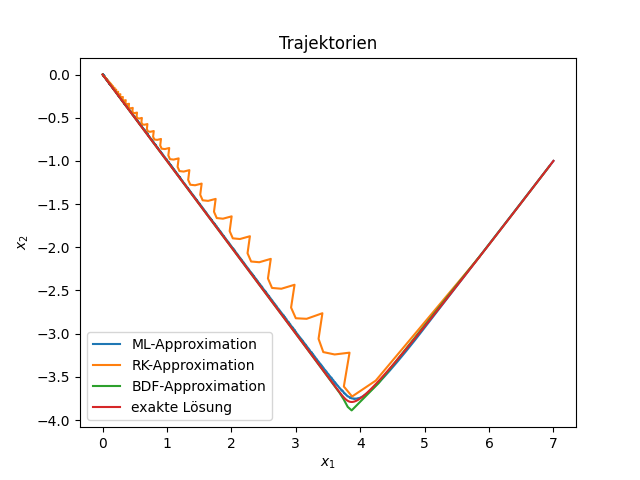
\includegraphics[scale=0.9]{Stiff_plots/stifftrajectories_}
       \caption{Trajektorie des steifen Anfangswertproblems.}
       \label{fig:stiff-trajectories}
\end{figure}
\begin{figure}
       \centering
       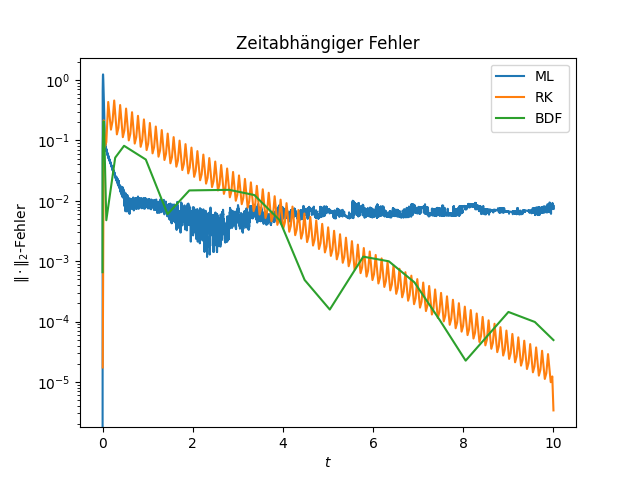
\includegraphics[scale=0.9]{Stiff_plots/stiffError_in_time}
       \caption{Globaler Fehler $\left\lVert x(t_i) - u_{\alpha}(t_i) \right\rVert_2$ der jeweiligen Verfahren
              mit $\alpha=\text{BDF}, \text{RK}, \text{ML}$ in Abhängigkeit der Zeit.}
       \label{fig:stiff-error-in-time}
\end{figure}
Der oszillierende Fehler des Runge-Kutta-Verfahrens stimmt mit dem Verhalten der Trajektorie überein. Des Weiteren fällt
auf, dass der Fehler des neuronalen Netzes über die Zeit nahezu konstant bleibt, während der Fehler der anderen
Verfahren im Laufe der Zeit sinkt. Zudem sehen wir in \ref{fig:stiff-error} und \ref{fig:stiff-loss} den Verlauf des
globalen Fehlers und der Kostenfunktion für steigende Epochen.
\begin{figure}
       \centering
       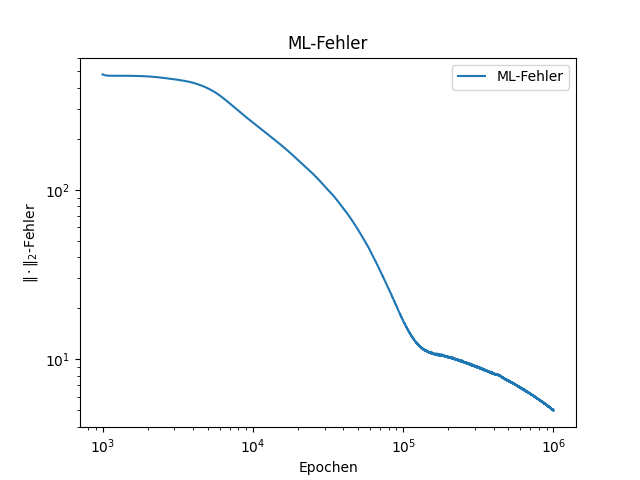
\includegraphics[scale=0.9]{Stiff_plots/stiffML_error_}
       \caption{Globaler Fehler für steigende Epochen.}
       \label{fig:stiff-error}
\end{figure}
\begin{figure}
       \centering
       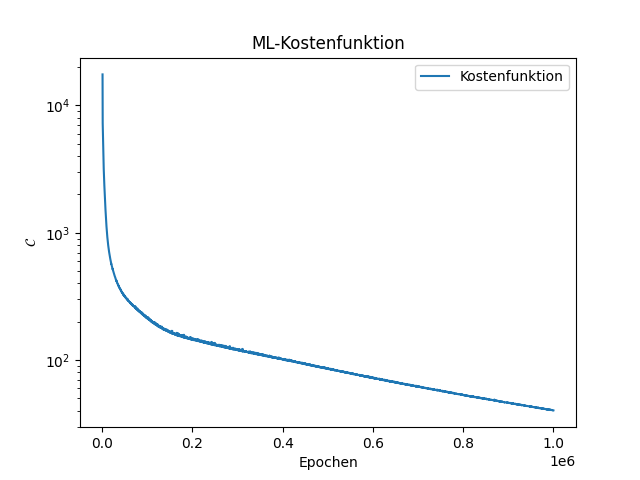
\includegraphics[scale=0.9]{Stiff_plots/stiffML_Loss_}
       \caption{Kostenfunktion für steigende Epochen.}
       \label{fig:stiff-loss}
\end{figure}
Sowohl der globale Fehler als auch die Kostenfunktion sinken wie erwartet bei steigender Epchenzahl, jedoch wird die
Steigung beider Graphen betragsmäßig kleiner. Um eine genauere Approximation zu erhalten, müssten wir die Anzahl der
Epochen erhöhen, wobei dies zu einer Laufzeit von über $\approx 2.2$ Stunden führen würde. Das BDF-Verfahren hat
trotz einer Beschränkung der globalen und relativen Toleranz das Anfangswertproblem in $0.039$ Sekunden mit akzeptablen
Fehler gelöst. Deshalb können wir zusammenfassend sagen, dass das BDF-Verfahren allgemein qualifizierter ist zur Lösung
von steifen Anfangswertproblemen.

\subsection{Harmonischer Oszillator}
\label{sec:harmonischer-oszillator}
Zuletzt werden wir die Lösung für den harmonischen Oszillator mit verschiedenen Netzwerkstrukturen approximieren und
die Ergebnisse untereinander und mit dem 4-5-Runge-Kutta-Verfahren vergleichen. Die Bewegung eines harmonischen
Oszillators ist gegeben mit
\begin{align}
       \label{harmonic-oscillator}
       &x^{\prime}=v, \qquad v^{\prime}=-\frac{k}{m}x, \\
       &x(0)=v(0)=0, \nonumber
\end{align}
wobei zur Vereinfachung $m=1$ gesetzt wird. Außerdem gilt für das numerische Verfahren $k=1$. Tabelle
\ref{stiff-table-data} enthält alle Daten, welche für alle folgenden neuronale Netze verwendet werden.
\begin{table}
       \renewcommand{\arraystretch}{1.0}
       \centering
       \begin{tabular}{ l | l }
              \hline
              Hyperparameter und Initialisierungsintervalle & \\
              \hline
              Anfangswertbereiche &
              $(x_{0},v_0) \in [-1.0, 1.0] \times [-1.0, 1.0]$ \\
              Paramaterbereiche & $k \in [0.5, 2.0]$ \\
              Zeitraum & $t \in [0, 2\pi]$ \\
              \hline
              Optimierung & \\
              \hline
              Gradientenverfahren & Adam \\
              Gewichtsfunktion & $b(t)=1$ \\
              Batchsize & $|B|=10000$ \\
              Epochen & $1000000$ \\
              Gewichtsinitialisierung & Xavier-Initialisierung \\
              \hline
       \end{tabular}
       \caption{Hyperparameter, Initialisierungsintervalle und Optimierungsparameter für den harmonischen Oszillator
       \eqref{harmonic-oscillator}.}
       \label{stiff-table-data}
\end{table}
Wir werden zuerst eine konstante Anzahl Schichten $L=6$ und learning rate $\eta=0.0001$ verwenden und die Anzahl der
Neuronen pro Schicht variieren. Dazu betrachten wir versteckte Schichten mit den Längen
$n^{(l)} = 4,8,16,32$, $l = 1, \dots, L-1$. Tabelle \ref{stiff-table-first} enthält die genauen Netzwerkstrukturen.
\begin{table}
       \renewcommand{\arraystretch}{1.0}
       \centering
       \begin{tabular}{ l | l }
              \hline
              Netzwerk 1 & \\
              \hline
              Anzahl der Schichten & $L=6$ \\
              Eingabeschicht & $n^{(0)}=4$ mit $\Phi(x)=\tanh(x)$ \\
              versteckte Schichten & $n^{(l)}=4$, $l = 1, \dots, L-1$ mit $\Phi(x)=\tanh(x)$ \\
              Ausgabeschicht & $n^{(L)}=2$ mit $\Phi(x)=x$ \\
              learning rate & $\eta=0.0001$ \\
              Trainingrate & xx \\
              Traningszeit & xx Stunden \\
              \hline
              Netzwerk 2 & \\
              \hline
              Anzahl der Schichten & $L=6$ \\
              Eingabeschicht & $n^{(0)}=4$ mit $\Phi(x)=\tanh(x)$ \\
              versteckte Schichten & $n^{(l)}=8$, $l = 1, \dots, L-1$ mit $\Phi(x)=\tanh(x)$ \\
              Ausgabeschicht & $n^{(L)}=2$ mit $\Phi(x)=x$ \\
              learning rate & $\eta=0.0001$ \\
              Trainingrate & xx \\
              Trainingszeit & xx Stunden \\
              \hline
              Netzwerk 3 & \\
              \hline
              Anzahl der Schichten & $L=6$ \\
              Eingabeschicht & $n^{(0)}=4$ mit $\Phi(x)=\tanh(x)$ \\
              versteckte Schichten & $n^{(l)}=16$, $l = 1, \dots, L-1$ mit $\Phi(x)=\tanh(x)$ \\
              Ausgabeschicht & $n^{(L)}=2$ mit $\Phi(x)=x$ \\
              learning rate & $\eta=0.0001$ \\
              Trainingrate & xx \\
              Trainingszeit & xx Stunden \\
              \hline
              Netzwerk 4 & \\
              \hline
              Anzahl der Schichten & $L=6$ \\
              Eingabeschicht & $n^{(0)}=4$ mit $\Phi(x)=\tanh(x)$ \\
              versteckte Schichten & $n^{(l)}=32$, $l = 1, \dots, L-1$ mit $\Phi(x)=\tanh(x)$ \\
              Ausgabeschicht & $n^{(L)}=2$ mit $\Phi(x)=x$ \\
              learning rate & $\eta=0.0001$ \\
              Trainingrate & xx \\
              Trainingszeit & xx Stunden \\
              \hline
       \end{tabular}
       \caption{Netzwerkstrukuren der ersten Variation.}
       \label{stiff-table-first}
\end{table}
!TODO:Bilder!
\begin{figure}
       \centering
       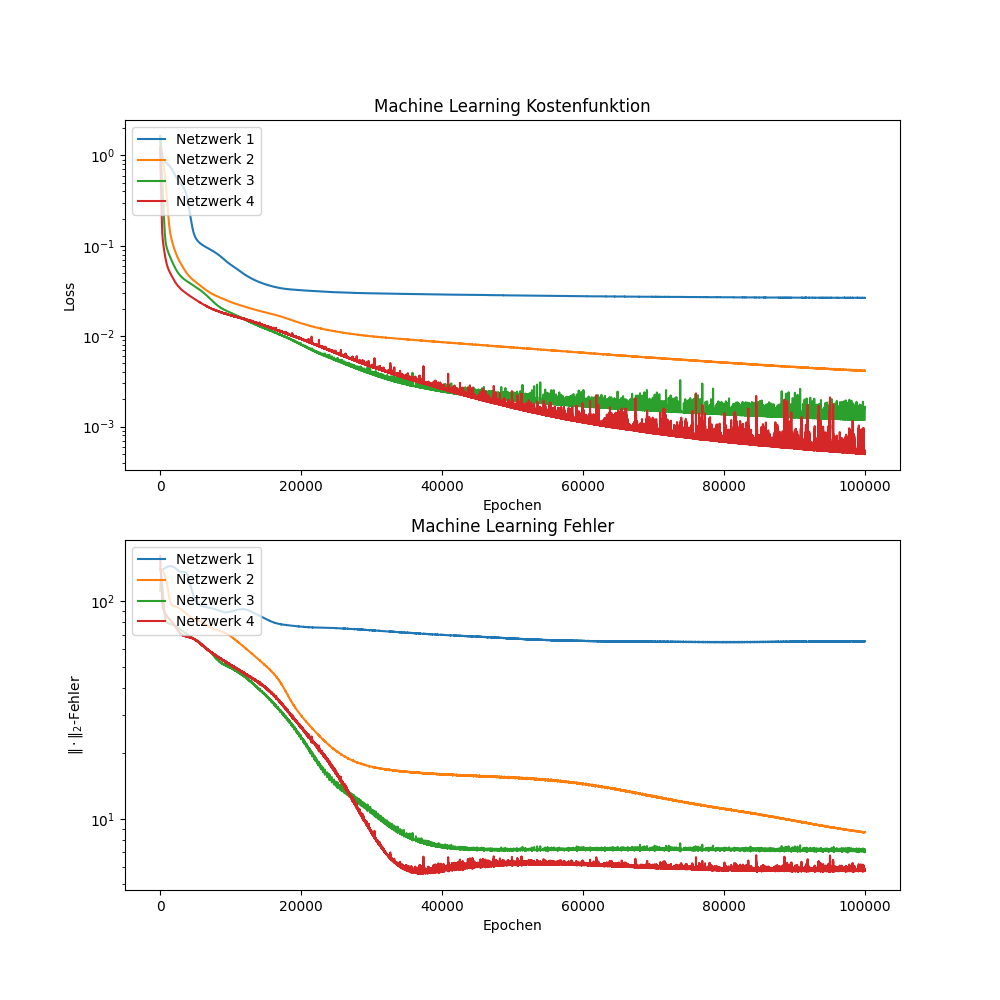
\includegraphics[scale=0.6]{harmonicoscillatorML_error__neurons_var_loss_and_error}
       \caption{Kostenfunktion und $\left\lVert \cdot \right\rVert_2$-Fehler der verschiedenen neuronalen Netze.}
       \label{fig:harmonic-neurons-variable-loss-error}
\end{figure}
Zuletzt werden wir Netzwerke mit 4, 8 und 16 versteckte Schichten vergleichen. Dazu wird die Länge der jeweiligen
Schichten$n^{(l)}=16$ und die learning rate $\eta=0.0001$ festgelegt. Genauere Angaben zu den Netzwerken befinden sich in
Tabelle
\ref{stiff-table-second}.
\begin{table}
       \renewcommand{\arraystretch}{1.0}
       \centering
       \begin{tabular}{ l | l }
              \hline
              Netzwerk 1 & \\
              \hline
              Anzahl der Schichten & $L=6$ \\
              Eingabeschicht & $n^{(0)}=4$ mit $\Phi(x)=\tanh(x)$ \\
              versteckte Schichten & $n^{(l)}=16$, $l = 1, \dots, L-1$ mit $\Phi(x)=\tanh(x)$ \\
              Ausgabeschicht & $n^{(L)}=2$ mit $\Phi(x)=x$ \\
              learning rate & $\eta=0.0001$ \\
              Trainingrate & xx \\
              Traningszeit & xx Stunden \\
              \hline
              Netzwerk 2 & \\
              \hline
              Anzahl der Schichten & $L=10$ \\
              Eingabeschicht & $n^{(0)}=8$ mit $\Phi(x)=\tanh(x)$ \\
              versteckte Schichten & $n^{(l)}=16$, $l = 1, \dots, L-1$ mit $\Phi(x)=\tanh(x)$ \\
              Ausgabeschicht & $n^{(L)}=2$ mit $\Phi(x)=x$ \\
              learning rate & $\eta=0.0001$ \\
              Trainingrate & xx \\
              Traningszeit & xx Stunden \\
              \hline
              Netzwerk 3 & \\
              \hline
              Anzahl der Schichten & $L=18$ \\
              Eingabeschicht & $n^{(0)}=16$ mit $\Phi(x)=\tanh(x)$ \\
              versteckte Schichten & $n^{(l)}=16$, $l = 1, \dots, L-1$ mit $\Phi(x)=\tanh(x)$ \\
              Ausgabeschicht & $n^{(L)}=2$ mit $\Phi(x)=x$ \\
              learning rate & $\eta=0.0001$ \\
              Trainingrate & xx \\
              Traningszeit & xx Stunden \\
              \hline
       \end{tabular}
       \caption{Netzwerkstrukuren der zweiten Variation.}
       \label{stiff-table-second}
\end{table}
!TODO: Bilder!
\newpage
